%!TEX root=../main.tex


\section {The Zeeguu Ecosystem}
In this section we present a very high level architecture of a prototype of such an ubiquitous monitoring ecosystem as described in the previous section. It is built around a platform dubbed Zeeguu. Figure \ref{fig:architecture} presents a very simplified version of the Zeeguu platform and ecosystem.

\begin{figure}[h!]
	% \centering
	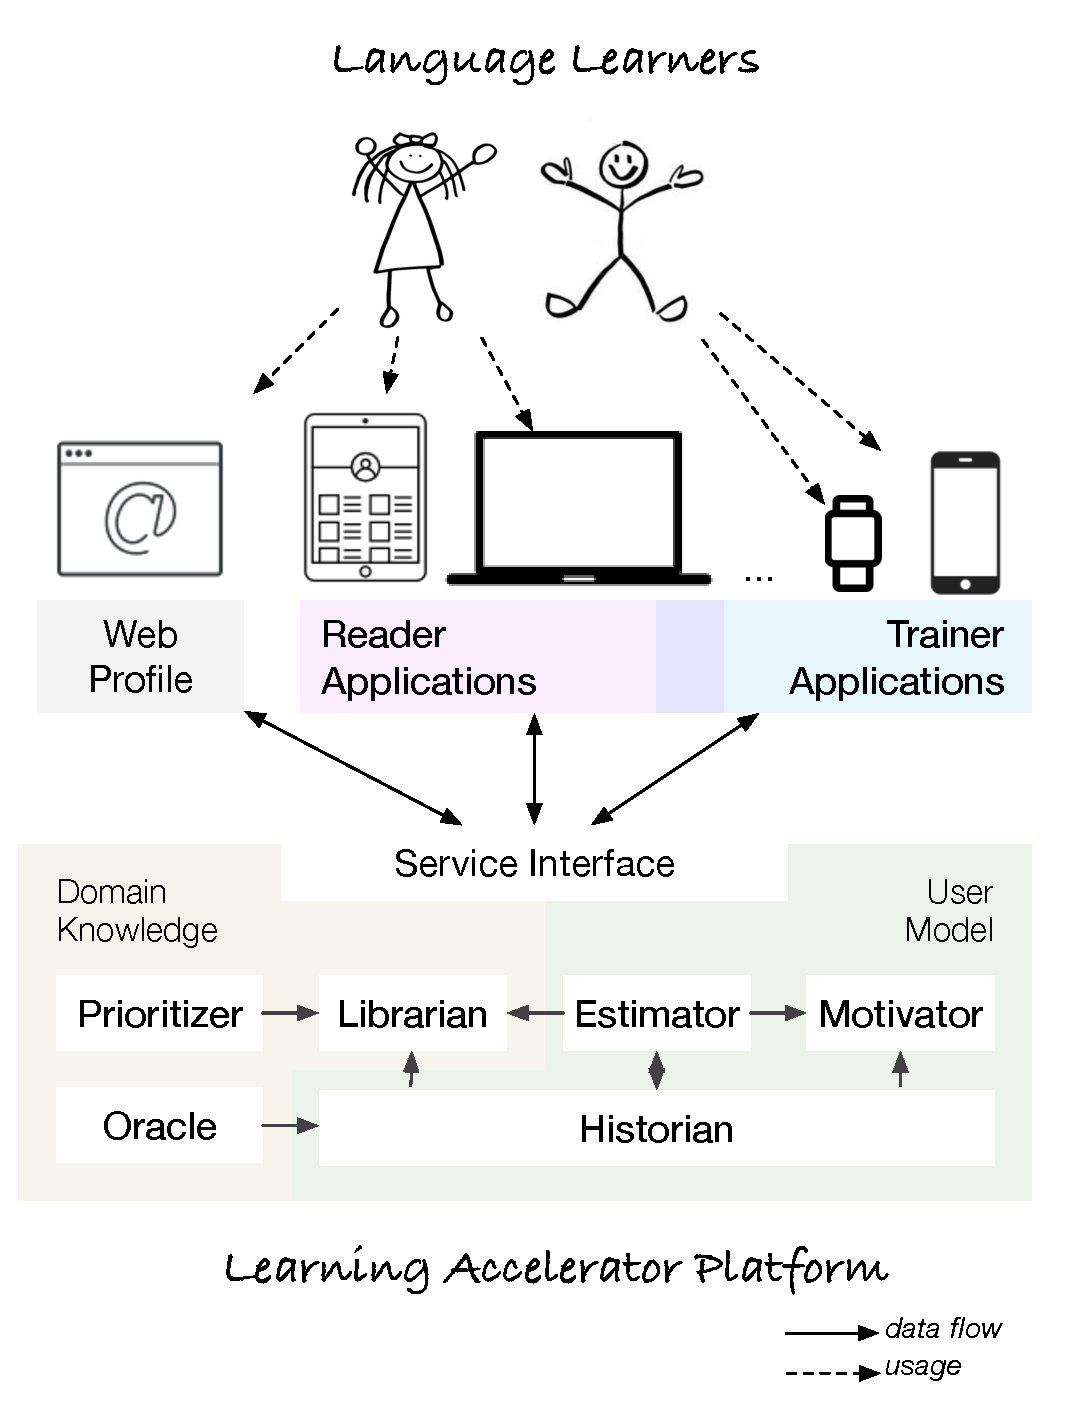
\includegraphics[width=\linewidth]{images/zeeguu-architecture.pdf}
	\caption{A very high-level view of the architecture of the Zeeguu ecosystem}
	\label{fig:architecture}
\end{figure}

The figure presents explicitly only one category of actors -- the {\em language learners}. A second type of actor in the ecosystem are the {\em applicatoin developers} who build the applications with which the learners interact. There are two types of such applications: 

\begin{description}
	
	\item {\bf Reader Applications} 
	support reading any kinds of materials in foreign languages. The reader applications must have two properties in common: 
		1) they should make it very convenient for the user to obtain translations for the texts he encounters in the foreign language. 
		2) they should report back to the platform every event that provides a hint to the current user knowledge. In particular, every word that is being translated by the user indicates his lack of knowledge with respect to that particular word, and every word that is not being translated by the user indicates their potential knowledge of that word.
	
		\item {\bf Trainer Applications} support the learner in practicing the vocabulary. A trainer application can request from the platform information on which words are prioritary to be studied. But a trainer application must also provide back to the platform information about how well the learner behaves with respect to a given word.

\end{description}

Note that as the Figure \ref{fig:architecture} subtly suggests by overlapping the two corresponding blocks, the Reader and the Trainer applications need not be disjoint applications, but one application could provide both functionalities.


The Zeeguu Platform is the core component of the learning ecosystem since it stores and orchestrates the exchange of information about the current and historical knowledge of the user. It needs to have several components, including: 

\newcommand {\archiblock}[1]{\item {\bf #1}}
\begin{enumerate}

		\archiblock{The Translator} is a service that provides translations between many pairs of languages to reader applications. It notifies the historian of every request it receives. 
		It uses adaptive strategies to choose between different backends that have different properties in terms of cost and quality.

		\archiblock{The Historian} is a data warehouse that sits at the core of a monitoring ecosystem. It records as much data as possible about all the interactions of a user with knowledge. 
		It has both relational and noSql components.
		% all the interactions of a learner with texts in the foreign language that are mediated by the Reader applications.

		\archiblock{The Oracle} is a machine learning based agent that {\em estimates the current knowledge of the learner} based on the information received from the Historian. It decides what are the most likely items that must be studied by the learner. 
		%
		\archiblock{The Prioritizer} is a data mining focused component which aims at ordering the information to be learned based on a global view of its importance. It can be built based on statistical analysis of the learning patterns of the various leaners or based on a generic study of corpora in the target language.


		\archiblock {The Librarian} is a web crawler that uses natural language processing techniques together with the information from the Oracle to support its goal of {\em providing recommendations to the learners} about which materials to study which are at the appropriate difficulty level as well as interesting enough for the learner.

		\archiblock {The Motivator} is an agent that uses gamification techniques to keep the learner motivated. It uses information from the Historian to be able to report on a learners engagement. It uses information from the Oracle to be able to provide feedback on the actual learning progress. 

\end{enumerate}



% Somewhere, we still have to discuss the question of: 
% - How are we going to maintain this ecosystem? who will provide the data storage and translation facilities for the long run? 
% - What are the incentives for new players to join the ecosystem?
% - ... 


